\section{Zielsetzung}
Das Geiger-Müller-Zählrohr wird zur Messung der Intentsität ionisierender und radioaktiver Strahlung verwendet.
Dabei erzeugt die Absorption der Strahlung einen messbaren elektrischen Impuls.
Es können $\alpha$- und $\beta$-Teilchen, sowie $\gamma$-Strahlung nachgewiesen und deren Intensiät gemessen werden.
\section{Theorie}
\subsection{Der Aufbau}
Hauptsächlich besteht das Geiger-Müller-Zählrohr aus einem metallischen Hohlzylinder und einem darin axial verlaufanden Draht.
Zwischen diesen beiden Elementen wird eine Spannung zwischen 300 - 2000 V angelegt, weshalb sie auch als Anodendraht mit dem  Radius $r_a$ und Kathodenzylinder mit dem Radius $r_k$ bezeichnet werden.
Im Innern des Zählrohrs befindet sich ein Gasgemisch aus einem Edelgas und Alkoholdämpfen. 
An einer Seite des Zylinders liegt ein Eintrittsfenster aus Mylar, welches aufgrund des Unterdrucks eingewölbt ist.
Des Weiteren ergibt sich durch die angelegte Spannung ein radialsymmetrisches elektrisches Feld mit der Feldstärke

\begin{equation}
    E (r) = \frac{U}{r \; \text{ln}\left(\frac{r_k}{r_a}\right)}.
\end{equation}

\begin{figure}[h]
    \centering
    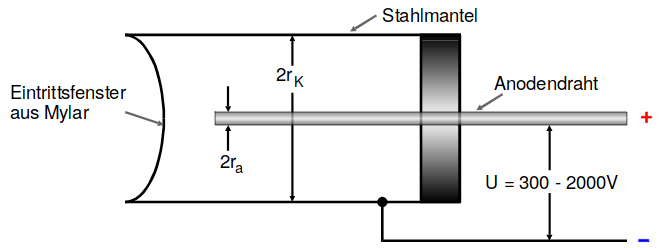
\includegraphics[height=4cm]{Theorie/Aufbau.png}
    \caption{Aufbau des Geiger-Müller-Zählrohrs.}
    \label{fig:aufbau}
\end{figure}

\subsection{Die Wirkungsweise}
Die Wirkungsweise des Geiger-Müller-Zählrohrs ist abhängig von der Spannung und lässt sich grundsätzlich in 5 verschiedene Bereiche einteilen.
Wenn ein zu detektierendes Teilchen in das Zählrohr eindringt, wird es absorbiert, indem dessen Energie für die Ionisation von Gasmolekülen verwendet wird.
Dabei entsteht bei jeder Ionisation ein Elektron und ein positives Ion.
Bei dieser Primärionisation ist die Energie des einfallenden Teilchens proportional zur Anzahl der entstehenden Elektronen.

\begin{figure}[h]
    \centering
    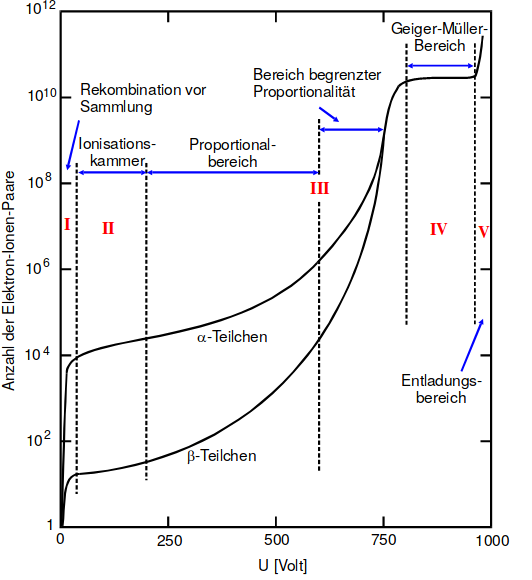
\includegraphics[height=10cm]{Theorie/wirkung.png}
    \caption{Abhängigkeit der Anzahl der Elektron-Ionen-Paare von der angelegten Spannung und die verschiedenenen Wirkungsbereiche.}
    \label{fig:wirkung}
\end{figure}

In Abbildung \ref{fig:wirkung} werden die verschiedenen Wirkungsbereiche des Geiger-Müller-Zählrohrs aufgezeigt.
Bei kleinen Spannungen im Bereich \textbf{I} geht ein Großteil der Elektronen-Ionen-Paare durch Rekombination verloren, da die Feldstärke zu gering ist. \\
Der Bereich \textbf{II} wird als Ionisationskammer bezeichnet, eine Vorstufe des Zählrohrs.
Dabei herrscht eine höherer Feldstärke, sodass praktisch alle gelösten Elektronen zum Anodendraht gelangen und gemessen werden.
In diesem Bereich liegt ein kontinuierlicher, aber sehr geringer Ionisationsstrom vor, der proportional zur Energie und Intensiät der zu messenden Strahlung ist.
Aufgrund des geringen Stroms ist die Ionisationskammer also nur bei hohen Strahlungsintensitäten einsetzbar. \\
Der Bereich \textbf{III} bildet den Proportionalitätsbereich.
Dabei können freie Elektronen aufgrund der hohen Feldstärke genug Energie aufnehmen um zusätzlich andere Elektronen aus den Edelgasmolekülen zu lösen.
Dieser Vorgang wird als Sto\ss{}ionisation bezeichnet und endet in einer Townsend-Lawine, die die lawinenartige Zunahme freier Elektronen beschreibt.
Dabei ist die am Anodendraht gesammelte Ladung $Q$ immer noch proportional zur Energie der einfallenden Strahlung.
Dieser Bereich wird deshalb auch als Proportionalitätszählrohr bezeichnet.\\
Das Geiger-Müller-Zählrohr bildet den Bereich \textbf{IV}.
Dieser Auslösebereich beschreibt den Bereich, in dem das ganze Zählrohrvolumen zur Intentsitätsmessung verwendet wird.
Das entsteht aufgrund der Anregung von Edelgasmolekülen durch hochenergetische freie Elektronen und der daraus resultierenden Aussendung von UV-Photonen, die sich anders als die Elektronen auch senkrecht zum elektrischen Feld ausbreiten können.
Diese UV-Photonen lösen im gesamten Zählrohr Townsend-Lawinen aus, was die Anzahl der freien Elektronen immens steigert.
Dadurch hängt die zu messende Intensität nur noch von der Betriebsspannung und dem Volumen des Zählrohrs ab.
Anders als bei der Ionisationskammer in Bereich \textbf{II} können die elektrischen Impulse nun mit geringem Aufwand gemessen und die Intenstiät der Strahlung bestimmt werden.
Allerdings ist eine Energiemessung aufgrund der räumlichen Ausbreitung im Geiger-Müller-Zählrohr nicht mehr möglich.

\subsection{Der Einfluss der positiven Ionen}
Der Ionisationsstrom wird anhand der freien Elektronen gemessen, die sich zum Anodendraht bewegen.
Dabei werden die entstehenden positiven Ionen zunächst vernachlässigt.
Allerding bleiben die Ionen aufgrund ihrer höheren Masse zwischen Kathodenzylinder und Anodendraht.
Dadurch wird das elektrische Feld so weit herabgesetzt, dass keine Sto\ss{}ionisation mehr möglich ist.
Diese Zeit wird auch als Totzeit $T$ bezeichnet.\\
Durch das elektrische Feld bewegen sich die Ionen zum Kathodenzylinder und werden dort neutralisiert.
Erst bei vollständiger Neutralisation wird wieder die gleiche Amplitude registriert.
Vorher wird noch eine Erholungszeit $T_E$ definiert, die den Zeitraum beschreibt, in dem die Ausgangsimpulse eine geringere Höhe haben, wie in Abbildung \ref{fig:Ionen} gezeigt wird.
 
\begin{figure}[h]
    \centering
    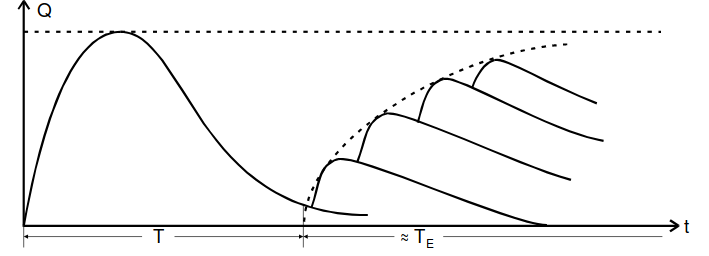
\includegraphics[height=4cm]{Theorie/Ionen.png}
    \caption{Tot- und Erholungszeit eines Zählrohrs im Zeit-Ladungs-Diagramm.}
    \label{fig:Ionen}
\end{figure}

Außerdem wird bei der Neutralisation der Ionen an dem Kathodenzylinder so viel Energie frei um Elektronen aus dem Metallmantel zu lösen.
So kann durch ein einfallendes Teilchen ein weiterer zeitversetzter elektrischer Impuls registriert werden.
Dieser Vorgang wird als Nachentladung beschrieben.
Dabei entspricht die zeitliche Differenz der beiden Impulse $T_L$ die Zeit, in der das Ion von seinem Entstehungsort zum Kathodenzylinder gewandert ist.
Da $T_L$ größer ist als die Totzeit $T$, könnte es zu schlechten Messergebnissen in der nächsten Messreihe führen.
Um dem entgegenzuwirken, werden Alkoholdämpfe in das Zählrohr eingebracht.
Dies dient dazu, dass die positiven Ionen ihre Energie an die Alkoholmoleküle abgegen.
Die Alkoholmoleküle werden dadurch ionisiert und wandern zum Metallmantel, wo sie allerdings nicht genug Energie aufbringen können um ein Elektron zu lösen.
Dabei wird keine Nachentladung registriert und die Messwerte werden nicht verfälscht.

\subsection{Charakteristik des Zählrohrs}
Die Charakteristik des Zählrohrs wird in Abbildung \ref{fig:char} dargestellt.
Bei der Spannung $U_E$ setzt der Auslösebereich ein.
Das darauf folgende Plateau hat eine hohe Aussagekraft über die Qualität des Zählrohrs.
Je flacher und länger das Plateau, desto höher ist die Qualität der Zählrohrs.
Die Steigung wird durch Nachentladungen, die trotz des Alkoholdampfes entstehen, hervorgerrufen.
Die Zahl der Nachentladung steigt am Ende des Plateaus sehr stark an.
Dadurch wird eine Dauerentladung gezündet, die in der Zerstörung des Zählrohrs enden kann.

\begin{figure}[h]
    \centering
    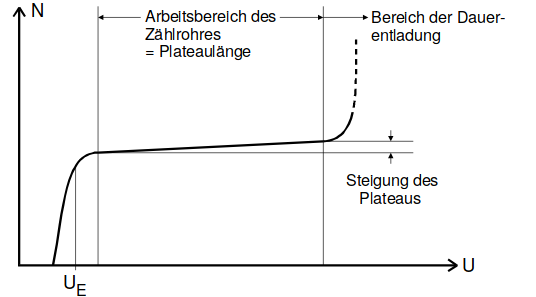
\includegraphics[height=6cm]{Theorie/char.png}
    \caption{Arbeitsbereich der Zählrohrs im Teilchen-Spannungsdiagramm.}
    \label{fig:char}
\end{figure}

\subsection{Ansprechvermögen des Zählrohrs}
Das Ansprechvermögen beschreibt mit welcher Wahrscheinlichkeit ein einfallendes Teilchen im Zählrohr registert wird.
Um das Ansprechvermögen zu optimieren besteht das Eintrittsfenster aus Mylar, einem dünnwandingen Material.
Wegen des hohen Ionisationsvermögens und der hohen Wechselwirkung mit Materie von $\alpha$- und $\beta$-Strahlung liegt deren Ansprechvermögen bei nahezu $100\%$.
Bei Photonen ist es vergleichsweise gering mit einem Ansprechvermögen von $1\%$.
Das liegt an der geringen Wechselwirkung mit Materie.